%!TEX root = ../template.tex
%%%%%%%%%%%%%%%%%%%%%%%%%%%%%%%%%%%%%%%%%%%%%%%%%%%%%%%%%%%%%%%%%%%
%% chapter1.tex
%% NOVA thesis document file
%%
%% Chapter with introduction
%%%%%%%%%%%%%%%%%%%%%%%%%%%%%%%%%%%%%%%%%%%%%%%%%%%%%%%%%%%%%%%%%%%

\typeout{NT FILE chapter1.tex}%

\chapter{Introduction}
\label{cha:introduction}









































%Excertos de coisas que estavam no template versão original



%\prependtographicspath{{Chapters/Figures/Covers/}}

% epigraph configuration
%\epigraphfontsize{\small\itshape}
%\setlength\epigraphwidth{12.5cm}
%\setlength\epigraphrule{0pt}

%
\includegraphics[width=0.1\linewidth]{NOVAthesisFiles/Images/novathesis-insignia}\hfill
%
\includegraphics[width=0.875\linewidth]{NOVAthesisFiles/Images/novathesis-text}

% \noindent This is the \gls{novathesis} \LaTeX\ template \ntindex[Template!]{Version} \novathesisversion\ from   {Template!date}\novathesisdate.

% \epigraph{
%   This work is licensed under the \href{https://www.latex-project.org/lppl/lppl-1-3c/}{\LaTeX\ Project Public License v1.3c}.
%   To view a copy of this \ntindex[Template!]{license}, visit the \href{https://www.latex-project.org/lppl/}{LaTeX project public license}.
% }

% \section{Welcome to the \novathesis\ Template}
% \label{sec:if_you_use_this_template}

%~\ref{cha:users_manual}.

% \subsection{Your Time is Precious}
% \label{sub:time_is_money}

%\emph{learning the rules} 

%\begin{tcolorbox}[colback=green!8]
%\\\parbox{\linewidth}{\raggedleft---~\emph{João Lourenço}}
%\end{tcolorbox}

%\href{https://www.paypal.com/donate/?hosted_button_id=8WA8FRVMB78W8}{\fcolorbox{DarkGreen}{gray!15}{\textbf{~HERE~}}} 


% \begin{figure}[htbp]
%     \centering
%     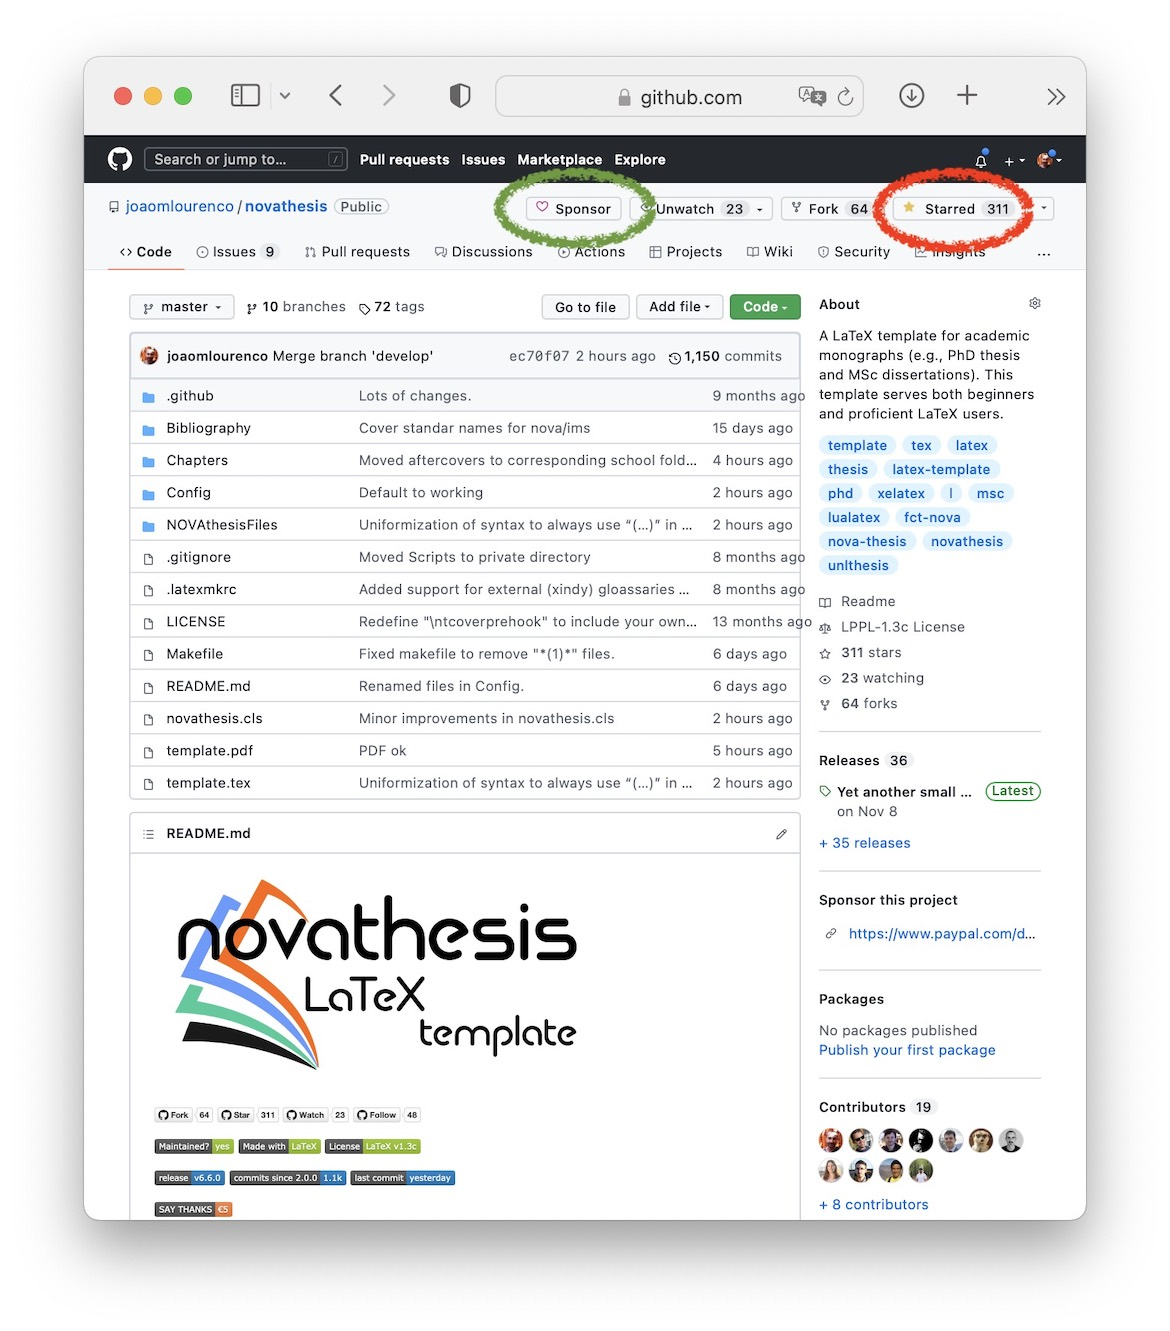
\includegraphics[width=0.5\linewidth]{github1}
%     \caption{The \gls{novathesis} project web page in GitHub.}
%     \label{fig:github}
% \end{figure}

% \section{The \emph{NOVAthesis} Template}
% \label{sec:a_bit_of_history}

% \ntindex[Template]{}

% \newenvironment{ntUniversity}[1]{
%   \renewcommand\tabularxcolumn[1]{m{##1}}% for vertical centering text in X column
%   % \renewcommand\cellgape{\Gape[1cm]}
%   % \setcellgapes{20pt}
%   % \makegapedcells
%   % % \setlength{\extrarowheight}{20pt}
%   % \renewcommand{\arraystretch}{2}
%   \rowcolors{1}{}{GhostWhite}
%     \xltabular{\linewidth}{cX}%
%       \caption{#1's Schools supported by the \gls{novathesis} template\label{tab:supported_schools_#1}}\\
%     \toprule%
%     \rowcolor{Gainsboro}%
%     & \Gape[1.5ex]{\thead[l]{#1}}\\
%     \midrule%
% }{%
%     \bottomrule
%     \endxltabular%
% }

% \makeatletter
% \newtoggle{coverspace}
% \newcommand{\docCover}[1]{%
%   \setlength{\fboxsep}{0pt}%
%   \togglefalse{coverspace}%
%     \Gape[1.5ex]{\begin{mcellbox}[cc]
%     \@for\myi:=#1\do{%
%       \fbox{\colorbox{White}{\includegraphics[align=c,width=1.5cm]{1up/\myi}}}%
%         \ifx\@xfor@nextelement\@nnil
%           % last iteration
%         \else
%           % not last iteration
%           \iftoggle{coverspace}{\togglefalse{coverspace}\\\\[-14pt]}{\toggletrue{coverspace}~}%
%         \fi
%   }%
%     \end{mcellbox}}
% }
% \makeatother
% \newcommand{\schlName}[3]{\textbf{#1} (\href{#3}{#2})}
% \newcommand{\degreeName}[3]{\newline\null\quad • #1 \href{#3}{(#2)}}

% \begin{ntUniversity}{NOVA University Lisbon}
%   {
%       \docCover{nova-fct-phd-en,nova-fct-msc-en}
%   } &  {
%     \schlName{NOVA School of Science and Technology}{FCT-NOVA}{https://www.fct.unl.pt}
%     \degreeName{All PhD Programs}{PhD}{https://www.fct.unl.pt/en/education/phd-programmes}
%     \degreeName{All MSc Programs}{MSc}{https://www.fct.unl.pt/en/education/master-degrees}
%   }\\
%   
% \end{ntUniversity}

% \newdata*{schlname}
% \newdata*{schlurl}
% \schlname(ea):={School of Architecture}
% \schlurl(ea):={https://www.uminho.pt/EN/uminho/Units/schools-and-institutes/Pages/School-of-Architecture.aspx}
% \schlname(ec):={School of Sciences}
% \schlurl(ec):={https://www.uminho.pt/EN/uminho/Units/schools-and-institutes/Pages/school-of-sciences.aspx}



% \subsection{Using Overleaf}
% \label{sub:using_overleaf}

% \ntindex[Installation!Overleaf]{}
% \ntindex[Using!Overleaf]{}

% \newcommand{\Overleaf}{\href{https://www.overleaf.com?r=f5160636&rm=d&rs=b}{Overleaf}}

% \begin{wrapfigure}{r}{0.3\linewidth}
% % \vspace*{-10ex}
% 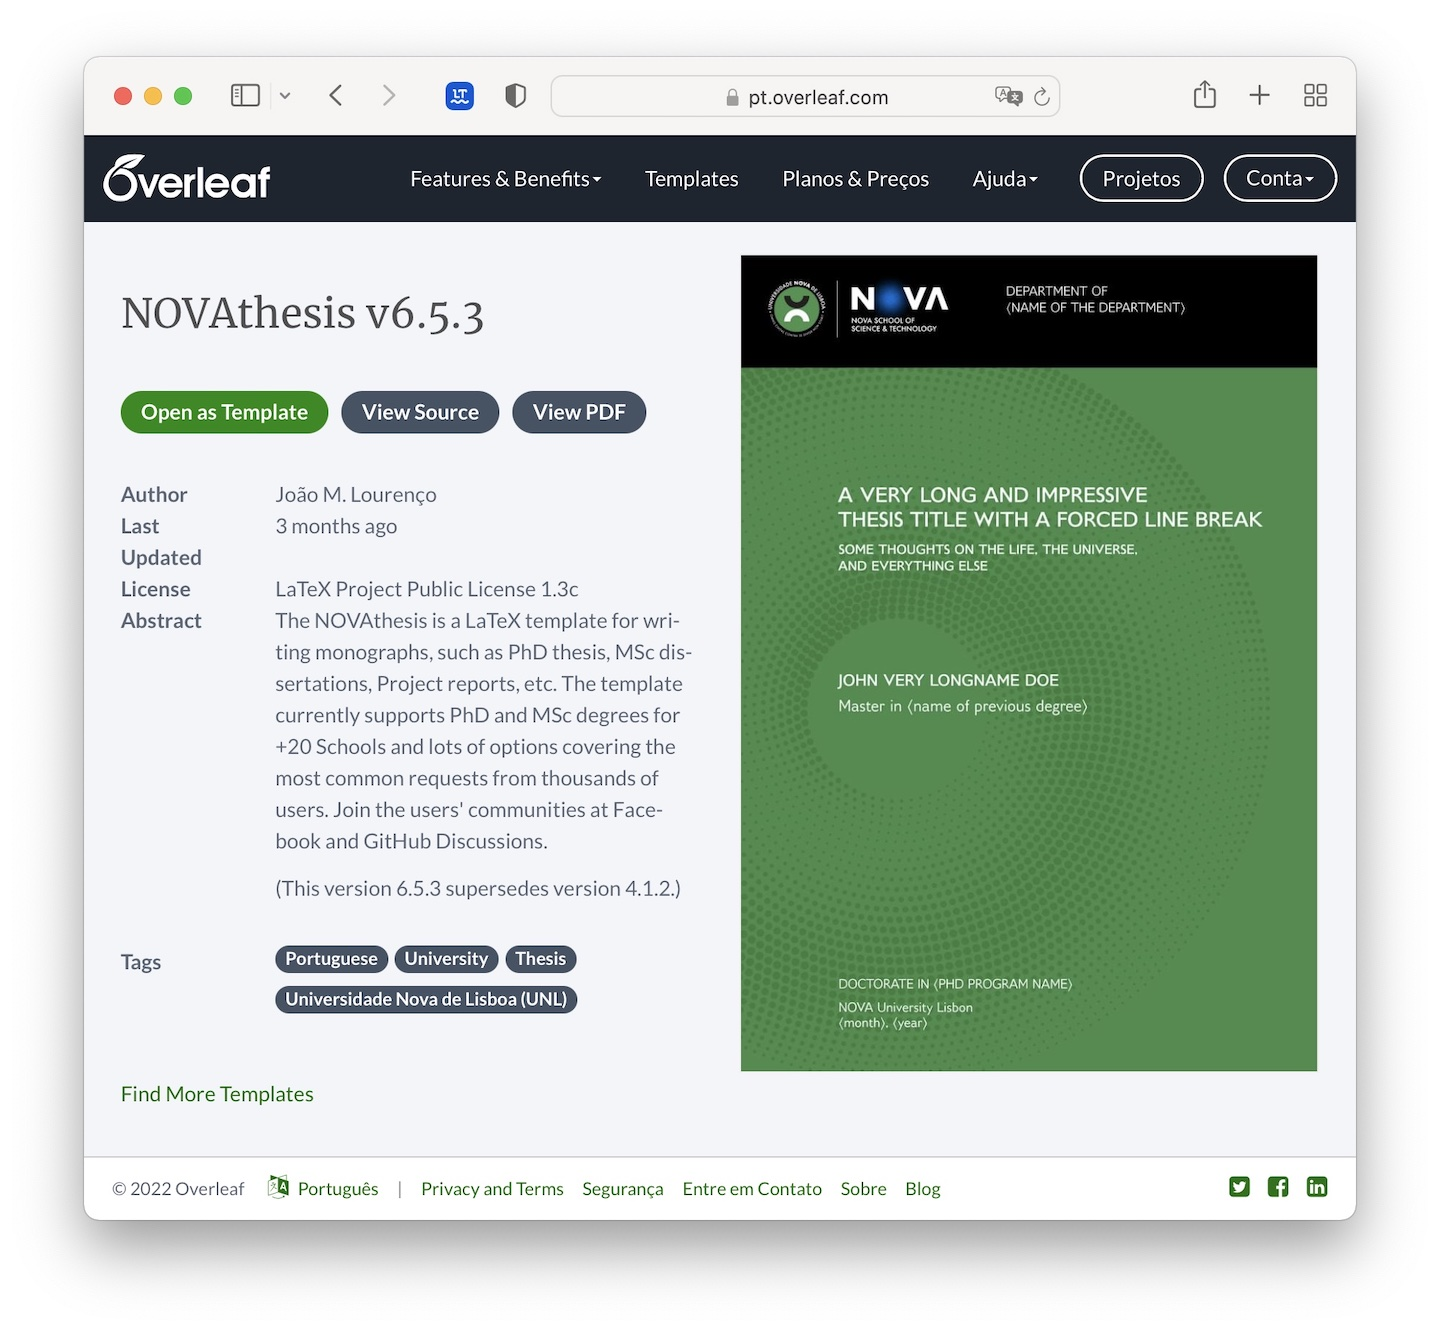
\includegraphics[width=\linewidth]{overleaf}%
% \caption{NOVAthesis template in Overleaf.}
% \label{fig:overleaf}
% \end{wrapfigure}
% \mbox{}\Overleaf\ is a collaborative cloud-based LaTeX editor used for writing, editing and publishing scientific documents. Like “Google Docs”,  

% \begin{tcolorbox}[colback=red!8]
% 	Notice that you need a (student) subscription to compile the \novathesis\ template in Overleaf, otherwise your compilation will always time out.
% \end{tcolorbox}

% \begin{description}
%   \item[Help:] If you just need some help, see above \Autoref{sec:getting_help}.
%   \item[Suggestion:] \ntindex[Suggestions]{} Do you have a suggestion/recommendation? Please add it to the wiki and help other users!
%   \item[Bug:] \ntindex[Bugs]{} Did you find a bug? Please open an issue. Thanks!
%   \item[New Feature:] \ntindex[Feature Requests]{} Would you like to request a new feature (or support of a new School)? Please open an issue. Thanks!

% \end{description}
